\documentclass[a4paper,12pt]{report}
\usepackage{subfigure}
\usepackage[utf8]{vietnam}
\usepackage[left=2.50cm, right=2.00cm, top=2.00cm, bottom=2.00cm]{geometry}
\usepackage{fancybox,graphicx}
\usepackage{mathrsfs} 
\usepackage{amsfonts}
\usepackage{longtable,array}
\usepackage{multirow}
\newlength\mylength
\newcolumntype{C}[1]{>{\centering\arraybackslash}p{#1}}
\usepackage[intlimits]{amsmath}
\usepackage{array}
\usepackage[unicode]{hyperref}
\usepackage{adjustbox}
% \usepackage{algorithm}
% \usepackage{algorithmicx}
\makeatletter
% \renewcommand{\ALG@name}{Thuật toán}
\makeatother
\usepackage{algpseudocode}
\usepackage{caption}
\usepackage{amsxtra,amssymb,latexsym,amscd,amsthm}
\usepackage{enumitem}
\usepackage{tikz}
\usepackage{makeidx}
\usepackage{float}
\usepackage{xcolor}
% \usepackage{lipsum}
% \usetikzlibrary{shapes.geometric}
% \usetikzlibrary{positioning,automata}
% \usepackage{scrextend}
% \usepackage{longfbox}
%Môi trường Lời giải
%\newtheorem{theorem}{Định lý}[chapter]
%\newtheorem{definition}{Định nghĩa}[chapter]
%\newtheorem{example}{Ví dụ}[chapter]
%\newtheorem{lemma}[theorem]{Bổ đề}
%Tiêu đề
% \newtheorem{pro}{Bài toán}
% \newtheorem*{constr}{Ràng buộc}
% \newtheorem*{calfunc}{Các hàm được thực thi}
% \newtheorem*{Sol}{Giải thuật}
% \newtheorem*{Anal}{Phân tích giải thuật}

% \usepackage{fancyhdr}
% \pagestyle{fancy}
% \lhead{}
% \chead{}
% \rhead{Nguyên lý Hệ Điều Hành}
% \lfoot{}
% \cfoot{\thepage}
% \rfoot{}

\paperheight=24cm
\paperwidth=17cm
\textwidth=13truecm
\textheight=19,7truecm
\topmargin=0cm
\headsep=20truept
\headheight=12pt
\voffset=-0.75truecm
\hoffset=-0.75cm
\oddsidemargin=0.5cm
\evensidemargin=0.5cm
\footskip=30 pt
\pagenumbering {arabic}
\setcounter{page}{1}
\setcounter{chapter}{0}
\addtocontents{toc}{\protect\vspace{20pt}}

\usepackage{xcolor}
\usepackage{listings}
\usepackage{titlesec}
\usepackage[bottom]{footmisc}

\titleformat{\chapter}[display]
{\normalfont\huge\bfseries}{\chaptertitlename\ \thechapter}{20pt}{\Huge}
\titlespacing*{\chapter}{0pt}{-50pt}{40pt}

% \renewcommand{\thechapter}{\Roman{chapter}}
% \renewcommand{\thesection}{\thechapter.\Roman{section}}
% \renewcommand{\thesubsection}{\thesection.\Roman{subsection}}

\definecolor{mGreen}{rgb}{0,0.6,0}
\definecolor{mGray}{rgb}{0.5,0.5,0.5}
\definecolor{mPurple}{rgb}{0.58,0,0.82}
\definecolor{backgroundColour}{rgb}{0.95,0.95,0.92}
\setcounter{secnumdepth}{4}
\setcounter{tocdepth}{4}

\lstdefinestyle{CStyle}{
	backgroundcolor=\color{backgroundColour},
	commentstyle=\color{mGreen},
	keywordstyle=\color{magenta},
	numberstyle=\tiny\color{mGray},
	stringstyle=\color{mPurple},
	basicstyle=\footnotesize,
	breakatwhitespace=false,
	breaklines=true,
	captionpos=b,
	keepspaces=true,
	numbers=left,
	numbersep=5pt,
	showspaces=false,
	showstringspaces=false,
	showtabs=false,
	tabsize=2,
	language=C
}


% \renewcommand{\fboxrule}{0.3pt}

\begin{document}

\thispagestyle{empty}

\begin{titlepage}
	\begin{figure}[h]
		\centering
		
\includegraphics[width=0.5\textwidth]{images/logotmh.png}
	\end{figure}

	\begin{center}
		\textbf{{\Huge CUỘC THI}} \\[10pt]
		\textbf{\LARGE TOÁN MÔ HÌNH 2023}\\[10pt]
		\textbf{\LARGE VÒNG 2}\\[10pt]
		\textbf{ 25 tháng 08 - 31 tháng 08, 2023}
		\\[3.0cm]

		\begin{tabular}{r l}
			\textbf{Tên đội thi}: &APM \\
			\textbf{Thành viên:}
				&$-$ Nguyễn Thành Phát \\
				&$-$ Lê Xuân An \\
				&$-$ Phạm Công Minh
		\end{tabular}
	\end{center}

	\vspace{\fill}
\end{titlepage}

\newpage

\tableofcontents
% \renewcommand{\thechapter}{\arabic{chapter}}
% \renewcommand{\thesection}{\thechapter.\arabic{section}}
% \renewcommand{\thesubsection}{\thesection.\arabic{subsection}}
% \newcounter{chapter}{0}

\chapter*{Thông tin cần thiết về các bài toán}
\addcontentsline{toc}{chapter}{Thông tin cần thiết về bài toán}

\section*{Danh sách các chữ viết tắt thuật ngữ}
\addcontentsline{toc}{section}{Danh sách các chữ viết tắt thuật ngữ}
\begin{flushleft}
	\begin{itemize}
		\item \textbf{count}: Số lượng giá trị được quan sát trong bài toán.

		\item \textbf{min}: Giá trị nhỏ nhất của tập dữ liệu.

		\item \textbf{max}: Giá trị lớn nhất của tập dữ liệu.

		\item \textbf{mean}: Giá trị trung bình của tập dữ liệu.
		\\
		Giá trị trung bình được cho bởi công thức dưới đây:
		$$
		mean = \frac{{\sum\limits_{i = 1}^{n} a_{i}}}{n}
		$$

		\item \textbf{std}: Độ lệch chuẩn của tập dữ liệu. Một độ lệch chuẩn cao sẽ cho thấy các giá trị trong tập dữ liệu quan sát được phân tán rộng lạc so với giá trị trung bình.
		\\
		Độ lệch chuẩn được cho bởi công thức dưới đây:
		$$
		std = \sigma = \sqrt{\frac{\sum\limits_{i = 1}^{n} (x_{i} - \bar{x})^{2}} {n}}
		$$

		\item \textbf{median}: giá trị trung vị, là giá trị nằm ở giữa tập dữ liệu sau khi đã được sắp xếp tăng dần.

		\item \textbf{outlier}: điểm dữ liệu ngoại lai, một điểm dữ liệu khác biệt đáng kể so với các điểm được quan sát khác. Một điểm dữ liệu ngoại lai có thể do sự thay đổi hoặc sai sót trong lúc đo đạc.

		\item \textbf{ha}: héc-ta (tiếng Việt), hectare (tiếng Anh).
	\end{itemize}
\end{flushleft}

\newpage

\chapter{Bài toán 1} % (fold)
\label{cha:bài_toán_1}
\section{Thống kê dữ liệu} % (fold)
\label{sec:thống_kê_dữ_liệu}
\begin{flushleft}
	Sau khi đã tham khảo các nguồn dữ liệu từ chương trình và một số nguồn dữ liệu ngoài, nhóm chúng tôi đã tổng hợp và thống kê tập dữ liệu về nạn mất rừng tại Việt Nam trong giai đoạn từ 2002 - 2020.

	\begin{figure}[H]
		\centering
		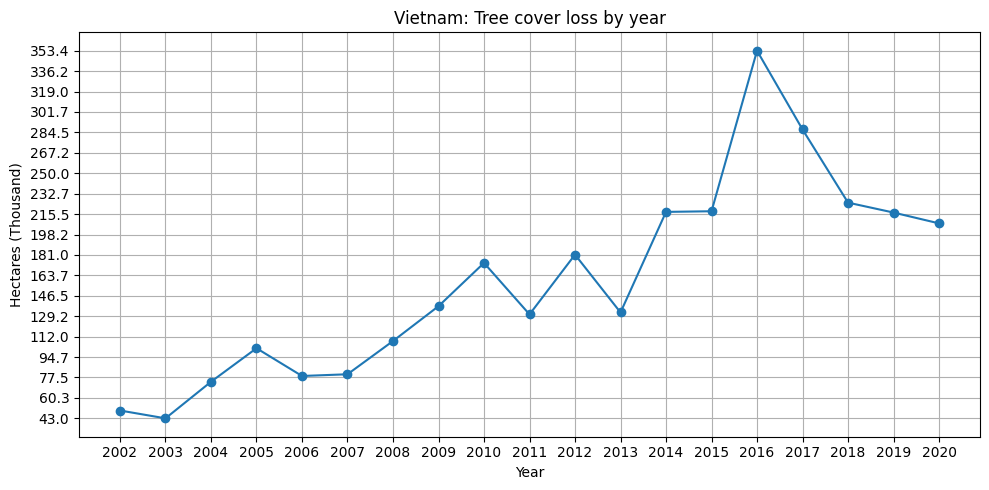
\includegraphics[width = 0.8\textwidth]{images/tree_cover_loss_by_year.png}
		\caption{Diện tích bao phủ rừng bị mất theo các năm}
	\end{figure}

	\begin{figure}[H]
		\centering
		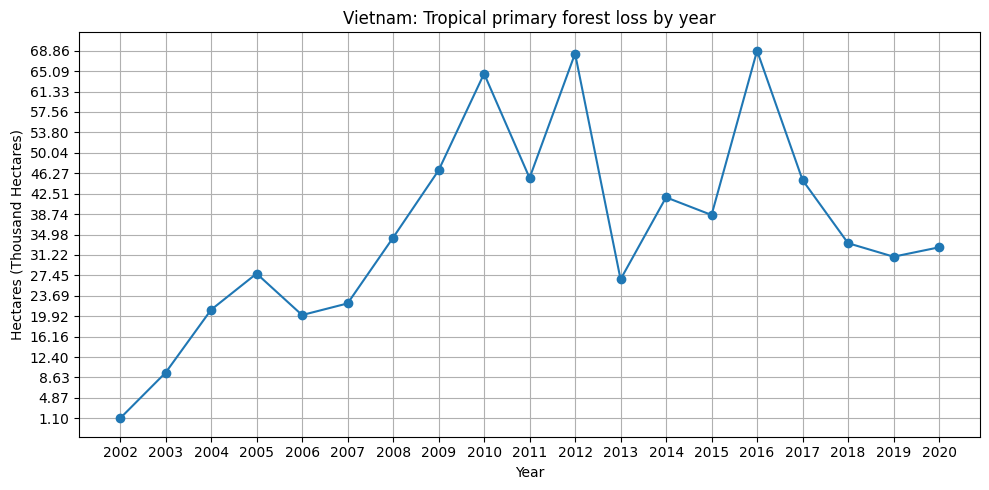
\includegraphics[width = 0.8\textwidth]{images/tropical_primary_forest_loss_by_year.png}
		\caption{Diện tích bao phủ rừng nguyên sinh bị mất theo các năm}
	\end{figure}
\end{flushleft}
% section mô_hình_hóa_dữ_liệu (end)

\section{Phân tích dữ liệu và mô tả các xu hướng} % (fold)
\label{sec:phân_tích_dữ_liệu_và_mô_tả_các_xu_hướng}
\begin{flushleft}
	Từ các mô hình số liệu ở trên, chúng ta hãy cùng phân tích sâu hơn và làm rõ các xu hướng của tập dữ liệu. \footnote{Chi tiết về hình ảnh minh họa và minh chứng xử lý số liệu cho thể tìm thấy ở notebook \textcolor{blue}{\underline{\href{https://github.com/XuananLe/MathModelingContest/blob/main/APM_TMH_V2/Problem1.ipynb}{Problem1.ipynb}}} của nhóm.}
	% \\[\baselineskip]
\end{flushleft}

\subsection{Phân tích dữ liệu} % (fold)
\label{sub:phân_tích_dữ_liệu}
\begin{flushleft}
	\begin{table}[H]
		\centering
		\begin{tabular}{|l|l|}
			\hline
			count & 19.00  \\
			\hline
			mean & 158.82  \\
			\hline
			std & 83.30  \\
			\hline
			min & 43.01  \\
			\hline
			max & 353.45  \\
			\hline
			median & 137.72  \\
			\hline
		\end{tabular}
		\caption{Các giá trị đặc trưng của diện tích bao phủ rừng thông thường}
	\end{table}

	Từ bảng trên chúng ta có thể thấy được:
	\begin{itemize}
		\item \textbf{count}: có 19 điểm dữ liệu được quan sát.

		\item \textbf{mean}: giá trị trung bình của tập dữ liệu $\approx$ 158.82.

		\item \textbf{std}: độ lệch chuẩn là 83.30. Một độ lệch chuẩn cao (như trong trường hợp này) cho thấy các giá trị trong tập dữ liệu phân tán rộng lạc so với giá trị trung bình.

		\item \textbf{min}: giá trị nhỏ nhất trong tập dữ liệu là 43.01.

		\item \textbf{max}: giá trị nhỏ nhất trong tập dữ liệu là 353.45.

		\item \textbf{median}: giá trị trung vị của tập dữ liệu là 137.72.
	\end{itemize}

	Nhìn chung, tập dữ liệu có sự phân tán khá lớn giữa giá trị thấp nhất và giá trị cao nhất với độ lệch chuẩn cao. Trung vị (137.72) thấp hơn giá trị trung bình (158.82), điều này có thể chỉ ra rằng tập dữ liệu có một số giá trị cao đặc biệt làm tăng giá trị trung bình.

	\begin{table}[H]
		\centering
		\begin{tabular}{|l|l|}
			\hline
			count & 19.00 \\
			\hline
			mean & 35.76 \\
			\hline
			std & 18.34 \\
			\hline
			min & 1.10 \\
			\hline
			max & 68.86 \\
			\hline
			median & 33.39 \\
			\hline
		\end{tabular}
		\caption{Các giá trị đặc trưng của diện tích bao phủ rừng nguyên sinh}
	\end{table}

	Từ bảng trên chúng ta có thể thấy được:
	\begin{itemize}
		\item \textbf{count}: có 19 điểm dữ liệu được quan sát.

		\item \textbf{mean}: giá trị trung bình của tập dữ liệu $\approx$ 35.76.

		\item \textbf{std}: độ lệch chuẩn là 18.34. Chỉ ra sự phân tán của dữ liệu với khoảng 18.34 đơn vị so với giá trị trung bình, dữ liệu phân tán tương đối.

		\item \textbf{min}: giá trị nhỏ nhất trong tập dữ liệu là 43.01.

		\item \textbf{max}: giá trị nhỏ nhất trong tập dữ liệu là 353.45.

		\item \textbf{median}: giá trị trung vị của tập dữ liệu là 137.72.
	\end{itemize}

	Từ các con số trên, chúng ta có thể rút ra được rằng:
	\begin{itemize}
		\item Phạm vi dữ liệu từ 1.1 đến 68.86 chỉ ra sự biến động lớn trong giá trị.

		\item Độ lệch chuẩn 18.34 cho thấy dữ liệu phân tán tương đối so với giá trị trung bình.

		\item Trung vị (33.39) thấp hơn giá trị trung bình (35.76 nghìn ha), điều này có thể chỉ ra rằng tập dữ liệu có một số giá trị cao đặc biệt làm tăng giá trị trung bình.
	\end{itemize}
\end{flushleft}
% subsection phân_tích_dữ_liệu (end)

\subsection{Phân tích và mô tả các xu hướng} % (fold)
\label{sub:phân_tích_và_mô_tả_các_xu_hướng}
\begin{flushleft}
	Để có thể nhìn rõ và phân tích các xu hướng của các tập dữ liệu được chính xác hơn, chúng ta sẽ sử dụng kĩ thuật rolling mean. Rolling mean, còn được gọi là moving average, là một phương pháp thống kê dùng để làm mượt một chuỗi thời gian hoặc chuỗi dữ liệu bằng cách tính trung bình liên tục của các giá trị trong một cửa sổ con có kích thước xác định. Rolling mean thường được dùng trong phân tích dữ liệu thời gian để giảm nhiễu và giúp làm nổi bật các xu hướng chung.
	\\[\baselineskip]

	Ví dụ, giả sử bạn có một chuỗi dữ liệu hàng ngày và bạn muốn tính rolling mean cho 7 ngày. Trong trường hợp này, giá trị rolling mean cho mỗi ngày sẽ được tính bằng cách lấy trung bình của giá trị đó và 6 ngày trước đó.
	\\[\baselineskip]

	\begin{figure}[H]
			\centering
			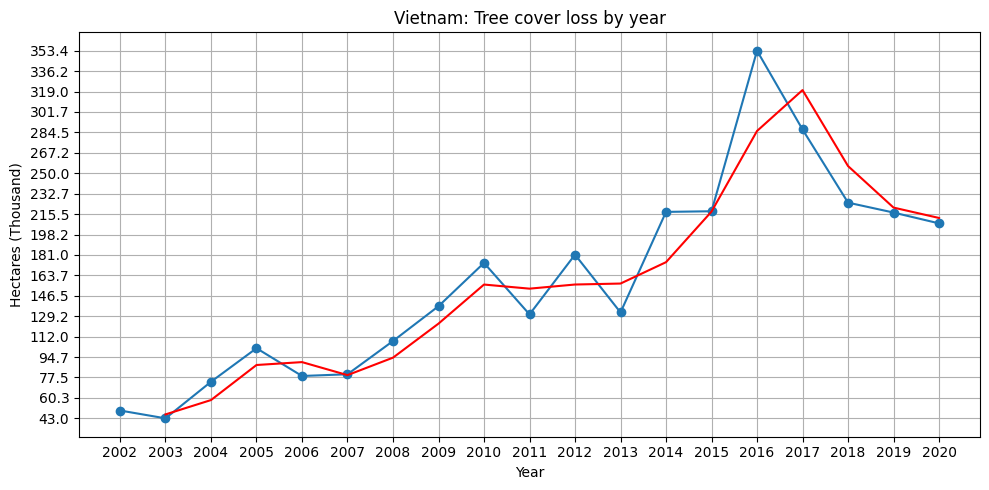
\includegraphics[width = \textwidth]{images/tree_cover_loss_by_year_rolling_mean.png}
			\caption{Áp dụng rolling mean lên tập dữ liệu 1}
	\end{figure}

	\begin{figure}[H]
			\centering
			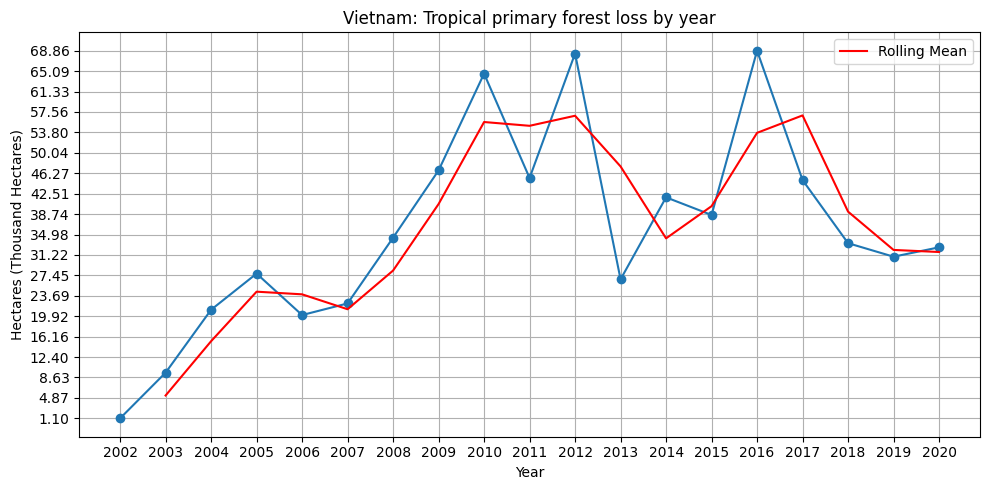
\includegraphics[width = \textwidth]{images/tropical_primary_forest_loss_by_year_rolling_mean.png}
			\caption{Áp dụng rolling mean lên tập dữ liệu 2}
	\end{figure}

	Ta thấy dữ liệu đã được làm mịn và thể hiện rõ các xu hướng cục bộ ở 2 tập dữ liệu. Bây giờ chúng ta sẽ tìm các xu hướng của 2 đồ thị này.

	\begin{figure}[H]
			\centering
			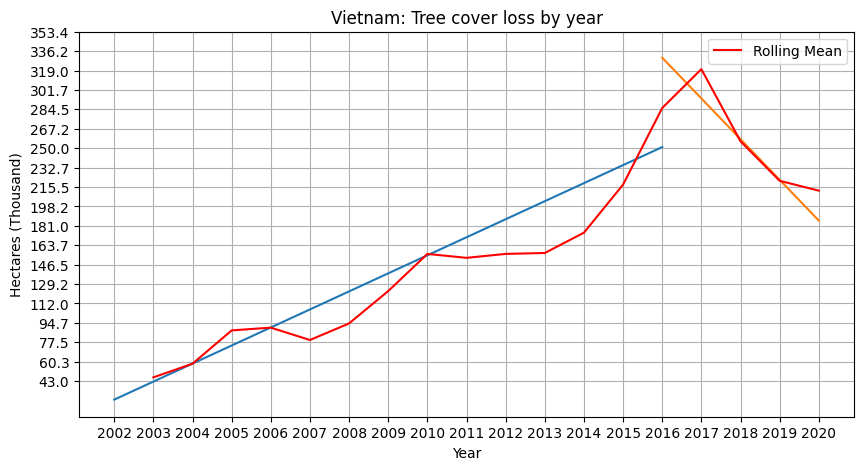
\includegraphics[width = \textwidth]{images/tree_cover_loss_by_year_trends_rolling_mean.png}
			\caption{Xu hướng biện động trên rolling mean của tập dữ liệu 1}
	\end{figure}

	\begin{figure}[H]
			\centering
			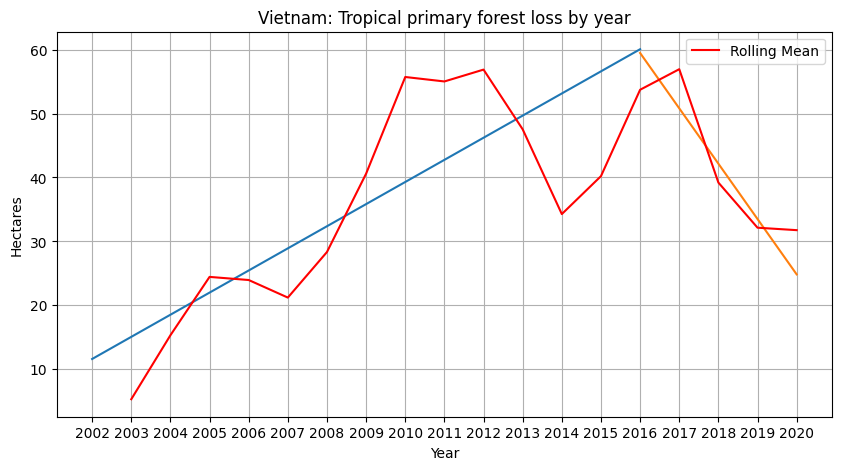
\includegraphics[width = \textwidth]{images/tropical_primary_forest_loss_by_year_trends_rolling_mean.png}
			\caption{Xu hướng biến động trên rolling mean của tập dữ liệu 2}
	\end{figure}

	\begin{figure}[H]
			\centering
			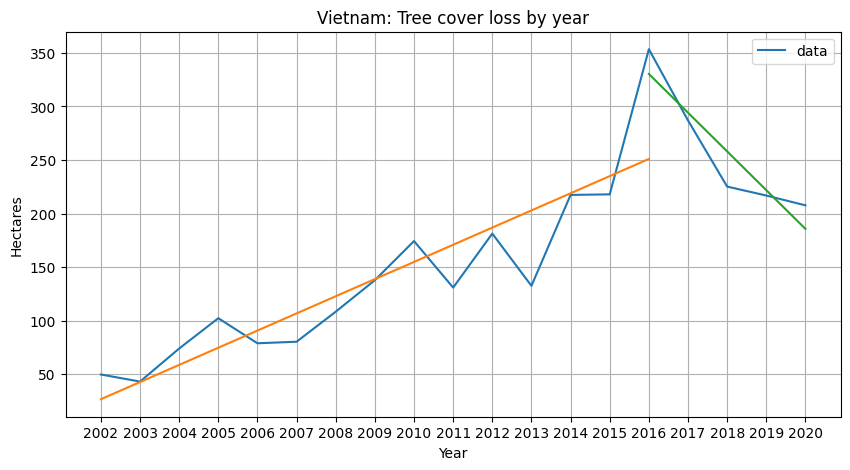
\includegraphics[width = \textwidth]{images/tree_cover_loss_by_year_trends.png}
			\caption{Các xu hướng biến động của diện tích bao phủ rừng bị mất}
	\end{figure}

	Nhìn chung thì nước ta có xu hướng mất rừng. Đầu tiên như trong hình trên chúng ta có thể thấy, có 2 giai đoạn mà diện tích rừng bao phủ bị mất thay đổi đột biến so với các năm trước. Năm diễn ra sự thay đổi là 2016 (135,5 nghìn hecta rừng bị mất). Đây chính là điểm outlier.
	\\[\baselineskip]

	\textbf{Xu hướng diễn ra sự tăng đột biến trước 2016 (2014 - 2016))}:
	\begin{itemize}
		\item Từ năm 2007 đến tháng 10/2010, cả nước xảy ra 10.444 vụ cháy rừng, gây thiệt hại 75.318ha rừng, bình quân mỗi năm bị cháy 5.380ha. Rừng bị cháy trong những năm gần đây chủ yếu là rừng trồng, với các loài cây chính là thông, tràm, bạch đàn, keo; đối với rừng tự nhiên, chủ yếu là cháy rừng nghèo kiệt, rừng khoanh nuôi tái sinh mới được phục hồi. Nguyên nhân chủ yếu trực tiếp gây ra cháy rừng là: Do đốt dọn thực bì làm nương rẫy, đốt dọn đồng ruộng gây cháy, chiếm 41,80\%; do người vào rừng dùng lửa để săn bắt chim thú, đốt đìa bắt cá, trăn, rùa, rắn…, hun khói lấy mật ong, chiếm 30,9\%; đốt dọn thực bì tìm phế liệu 6,1\%; cháy lân tinh 5,5\%; hút thuốc 3\%; đốt nhang 2\%; cố ý 5\%; nguyên nhân khác 5,7\%. \footnote{\textcolor{blue}{\underline{\href{http://www.kiemlam.org.vn/PortletBlank.aspx/89E2ECE261054E6DA2D06A694DE50016/View/So-12/TONG_QUAN_VE_BAO_VE_RUNG_VIET_NAM_VA_NHUNG_GIAI_PHAP_BAO_VE_RUNG/?print=904195979}{Tham khảo}}}}

		\item Nguyên nhân thứ hai có thể kể đến là hiện tượng hạn hán, xâm nhập mặn kéo dài do ảnh hưởng của hiện tượng El Nino bắt đầu từ 2014. \footnote{\textcolor{blue}{\underline{\href{https://nld.com.vn/thoi-su-quoc-te/el-nino-2014-manh-nhat-trong-nhieu-nam-20140505210910616.htm}{Tham khảo}}}}

		\item Nguyên nhân thứ ba có thể kể đến là do nạn khai thác rừng trái phép, đặc biệt là ở các tỉnh miền núi phía Bắc. \footnote{
			\textcolor{blue}{
			Tham khảo \underline{\href{https://dangcongsan.vn/phap-luat/nan-pha-rung-tang-dot-bien-o-dak-nong-313271.html}{1}}},
			\textcolor{blue}{\underline{\href{https://nhandan.vn/bao-dong-nan-pha-rung-o-bac-giang-post293931.html}{2}}},
			\textcolor{blue}{\underline{\href{https://baotintuc.vn/xa-hoi/bao-dong-do-nan-pha-rung-o-dien-bien-20150806175555226.htm}{3}}},
			\textcolor{blue}{\underline{\href{https://thanhnien.vn/pha-rung-tu-nhien-de-trong-cay-ngan-ngay-1851447176.htm}{4}}}
		}

		\item Nguyên nhân tiếp theo là khai thác sai về phương pháp do sai khác về phương pháp (tiêu chí các loại rừng) tính độ che phủ là 3,2\%, tương ứng 46.938,5 ha; do chuyển đổi mục đích sử dụng rừng... \footnote{\textcolor{blue}{\underline{\href{https://tuoitre.vn/giam-130000-ha-rung-co-quan-nao-chiu-trach-nhiem-684381.htm}{Tham khảo}}}}
	\end{itemize}

	Giai đoạn từ năm 2007 đến năm 2010 tuy không có biến động quá lớn về số rừng bao phủ bị mất nhưng vẫn có sự tăng lên đều. Điều này có thể được lý giải bằng việc nền kinh tế nước ta tăng trưởng vượt bậc trong giai đoạn này, đặc biệt là giai đoạn 2007-2008. Điều này dẫn đến việc nhu cầu về đất đai tăng lên, đặc biệt là đất đai có tiềm năng phát triển kinh tế cao. Điều này dẫn đến việc chuyển đổi mục đích sử dụng đất từ đất rừng sang đất trồng cây lâu năm.
	\\[\baselineskip]

	\textbf{Xu hướng giảm rõ rệt từ giai đoạn 2016 trở đi}:
	\begin{itemize}
		\item Tại giai đoạn năm 2016 trở đi, chúng ta tiếp tục thấy có sự chuyển biến mạnh nhưng lần này số lượng rừng được bao phủ đã tăng hơn 128291 ha rừng (tính tại năm 2018) so với điểm biến động năm 2016. Điều này có thể được lý giải bằng việc chính phủ đã có những chính sách hỗ trợ cho việc trồng rừng, bảo vệ rừng. Đặc biệt là việc chuyển đổi mục đích sử dụng đất từ đất rừng sang đất trồng cây lâu năm.
	\end{itemize}

	\begin{figure}[H]
			\centering
			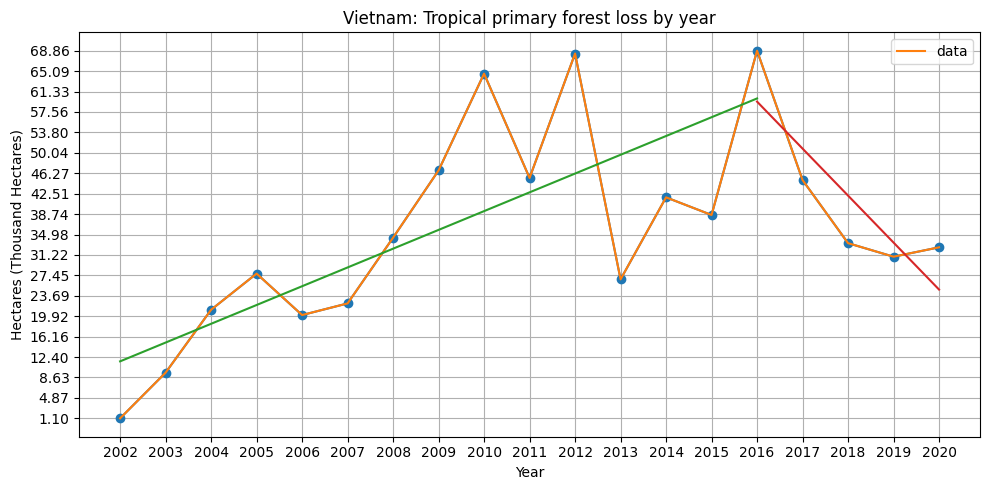
\includegraphics[width = \textwidth]{images/tropical_primary_forest_loss_by_year_trends.png}
			\caption{Các xu hướng biến động của diện tích bao phủ rừng nguyên sinh bị mất}
	\end{figure}

	Nhìn chung thì xu hướng tăng giảm diện tích bao phủ của rừng nguyên sinh gần tương đồng so với rừng bao phủ bình thường. Chúng ta từ năm 2007 đến năm 2010 có sự biến động khá mạnh nhưng đều trong việc mất rừng nguyên sinh (Trung bình mất hơn 13 nghìn ha rừng mỗi năm).
	\\[\baselineskip]

	\textbf{Xu hướng tăng của các năm trước 2016}:
	\begin{itemize}
		% \item Xu hướng tăng dần của các năm trước năm 2016 đều có các nguyên nhân về điều kiện khí hậu chung so với rừng thông thường.

		\item Mặc dù tổng diện tích rừng toàn quốc tăng trong những năm qua, nhưng diện tích rừng bị mất còn ở mức cao. Thống kê từ năm 1991 đến tháng 10/2008, tổng diện tích rừng bị mất là 399.118ha, bình quân 57.019ha/năm. Trong đó, diện tích được Nhà nước cho phép chuyển đổi mục đích sử dụng đất có rừng là 168.634ha; khai thác trắng rừng (chủ yếu là rừng trồng) theo kế hoạch hàng năm được duyệt là 135.175ha; rừng bị chặt phá trái phép là 68.662ha; thiệt hại do cháy rừng 25.393ha; thiệt hại do sinh vật hại rừng gây thiệt hại 828ha.

		\item Từ năm 2007 đến tháng 10 năm 2008, cả nước đã phát hiện, xử lý 494.875 vụ vi phạm các quy định của Nhà nước về quản lý, bảo vệ rừng và quản lý lâm sản.

		\item Do lợi nhuận cao từ buôn bán gỗ và động vật hoang dã trái phép, nên tình hình diễn ra phức tạp ở hầu khắp các địa phương.
	\end{itemize}

	\textbf{Xu hướng giảm đáng kể sau 2016}:
	\begin{itemize}
		\item Xu hướng năm 2016 đến năm 2020 có xu hướng giảm dần, điều này có thể là do các biện pháp chống phá rừng đã được thực hiện tốt hơn. Tuy nhiên, chúng ta vẫn cần phải cẩn trọng vì diện tích rừng bị mất vẫn còn ở mức cao. \footnote{
			\textcolor{blue}{
			Tham khảo \underline{\href{https://thuvienphapluat.vn/van-ban/Tai-nguyen-Moi-truong/Quyet-dinh-38-2016-QD-TTg-bao-ve-phat-trien-rung-dau-tu-ho-tro-ket-cau-ha-tang-cong-ty-nong-lam-nghiep-322052.aspx}{1}}},
			\textcolor{blue}{\underline{\href{https://thuvienphapluat.vn/van-ban/Linh-vuc-khac/Luat-lam-nghiep-367277.aspx}{2}}},
			\textcolor{blue}{\underline{\href{https://thuvienphapluat.vn/van-ban/Doanh-nghiep/Thong-tu-02-2018-TT-BKHDT-huong-dan-thuc-hien-Quyet-dinh-38-2016-QD-TTg-phat-trien-rung-381913.aspx}{3}}},
			\textcolor{blue}{\underline{\href{https://thuvienphapluat.vn/van-ban/Tai-nguyen-Moi-truong/Thong-tu-13-2019-TT-BNNPTNT-trong-rung-thay-the-khi-chuyen-muc-dich-su-dung-rung-427115.aspx}{4}}}
		}
	\end{itemize}
\end{flushleft}
% subsection phân_tích_và_mô_tả_các_xu_hướng (end)

% section phân_tích_dữ_liệu_và_mô_tả_các_xu_hướng (end)

% chapter bài_toán_1 (end)

\chapter{Bài toán 2} % (fold)
\label{cha:bài_toán_2}

\section{Hướng tiếp cận bài toán} % (fold)
\label{sec:tiếp_cận_bài_toán}
\begin{flushleft}
	Rừng chính là một trong những yếu tố giúp điều hòa và cân bằng khí hậu quan trọng nhất trên thế giới. Rừng giúp nuôi dưỡng đất, điều tiết nước, là nhà của khoảng 80\% các giống loài sống trên cạn, lọc không khí. Một khu vực không có rừng sẽ không thể có khí hậu ôn hòa cho con người và các loài sinh vật sinh sống. Chúng ta sẽ cùng xét mối liên hệ giữa độ bao phủ của rừng và mức khí thải $CO_{2}$ trong khắp cả nước ta để nói lên được vai trò của rừng. Có thể xem \textcolor{blue}{\underline{\href{https://github.com/XuananLe/MathModelingContest/blob/main/APM_TMH_V2/Problem2.ipynb}{Problem2.ipynb}}} của bài toán 2 trên github của nhóm.
	\\[\baselineskip]

	Đầu tiên, nhóm chúng tôi thử tiếp cận bài toán theo một mô hình toán học đơn giản, đó chính là hồi quy tuyến tính. Song, trong quá trình làm, chúng tôi đã nhận ra một điều quan trọng rằng, sự biến động phức tạp của lượng khí thải cũng như diện tích rừng phụ thuộc vào rất nhiều yếu tố và không thể xét qua một hàm hồi quy đơn giản. Do đó chúng tôi đã tìm hiểu về hệ phương trình vi phân thường và nhận thấy có thể biểu diễn mối liên hệ giữa 2 yếu tố trong bài toán có thể biểu diễn bằng cách này.

	\begin{figure}[H]
		\centering
		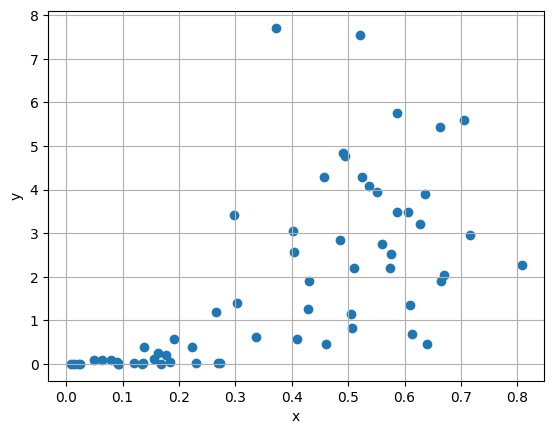
\includegraphics[width = 0.8\textwidth]{images/linear_problem2.png}
		\caption{Các điểm giá trị của bài toán 2}
	\end{figure}

	Như hình trên, các điểm giá trị quá rời rạc nhau và sẽ không thể tìm một đường thẳng tổng quát đi qua tất cả các điểm.
\end{flushleft}
% section tiếp_cận_bài_toán (end)

\section{Đề xuất phương án} % (fold)
\label{sec:đề_xuất_phương_án}
\begin{flushleft}
	Dưới đây là công thức do nhóm chúng tôi đề xuất để mô phỏng bài toán này:
	$$
		\frac{dR}{dt} = g \cdot R \cdot \left(1 - \frac{R}{K} \right) + a \cdot R \cdot C - \alpha \cdot r
	$$

	$$
		\frac{dC}{dt} = - \beta \cdot \frac{dR}{dt} + \gamma \cdot \frac{C}{R}
	$$

	Trong đó:
	\begin{itemize}
		\item $R$: diện tích bao phủ rừng.

		\item $C$: thể tích khí $CO_{2}$ thải ra.

		\item $t$: biến thời gian.

		\item $g$: tốc độ tăng trưởng tự nhiên của rừng.

		\item $K$: hằng số giới hạn diện tích tăng trưởng của rừng. Trong bài toán này chúng tôi đề xuất $K = 70\% \text{(diện tích Việt Nam)}$ vì diện tích rừng sẽ $\leq$ tổng diện tích đất.

		\item $r$: diện tích rừng bị mất đi do các yếu tố.

		\item $\alpha$: hệ số tốc độ mất rừng.

		\item $\beta$: tốc độ thải $CO_{2}$.

		\item $\gamma$: tốc độ kìm hãm mức thải $CO_{2}$.
	\end{itemize}

	Từng thành phần mang ý nghĩa như sau:
	\begin{itemize}
		\item $\frac{dR}{dt}$: tốc độ tăng trưởng rừng theo thời gian.
		\begin{itemize}
			\item $\frac{dR}{dt} \geq 0$: độ bao phủ rừng tăng hoặc không giảm.
			\item $\frac{dR}{dt} < 0$: độ bao phủ rừng giảm.
		\end{itemize}

		\item $\frac{dC}{dt}$: tốc độ xả thải $CO_{2}$.
		\begin{itemize}
			\item $\frac{dC}{dt} \geq 0$: tốc độ xả thải $CO_{2}$ tăng hoặc không giảm.
			\item $\frac{dC}{dt} < 0$: tốc độ xả thải $CO_{2}$ giảm.
		\end{itemize}

		\item $g \cdot R \cdot \left(1 - \frac{R}{K} \right)$: sự tăng trưởng tự nhiên của rừng. Hệ số $\left(1 - \frac{R}{K} \right)$ là giới hạn tốc độ tăng trưởng.

		\item $- \alpha \cdot r$: ảnh hưởng của con người, thiên tai đến độ bao phủ rừng.

		\item $a \cdot R \cdot C$: thể hiện chính sách trồng rừng của khu vực khi nhận thức được mức độ ảnh hưởng của $CO_{2}$.

		\item $- \beta \cdot \frac{dR}{dt}$: mức thải $CO_{2}$ có xu hướng giảm khi diện tích rừng tăng và ngược lại.

		\item $\gamma \cdot \frac{C}{R}$: mức thải $CO_{2}$ có thể tăng do con người ngày càng đông, càng nhiều nhà máy, phương tiện giao thông. Tuy nhiên sẽ tỉ lệ nghịch với diện tích rừng.
	\end{itemize}

	Với bài toán này, chúng tôi đề xuất các hệ số như sau và kèm theo các giả thiết dưới:
	\\

	Giả thiết:
	\begin{itemize}
		\item Không xét tới các yếu tố khí hậu cực đoan như thiên tai, hạn hán có thể gây ảnh hưởng đến diện tích bao phủ rừng.

		\item Không xét các chính sách ngăn chặn lâm tặc mới được cập nhật.

		\item Chỉ xét lượng $CO_{2}$ và tốc độ phát triển các nhà máy và phương tiện giao thông theo thời điểm làm bài toán này.
	\end{itemize}

	Các hệ số:
	\begin{itemize}
		\item $g$: 0.4

		\item $K$: $70\% \cdot 33169000$

		\item $a$: 80

		\item $\alpha$: 10

		\item $\beta$: 0.18

		\item $\gamma$: 0.9
	\end{itemize}

	Đây là kết quả của mô hình sau khi chạy với các điều kiện và tham số trên:
	\begin{figure}[H]
		\centering
		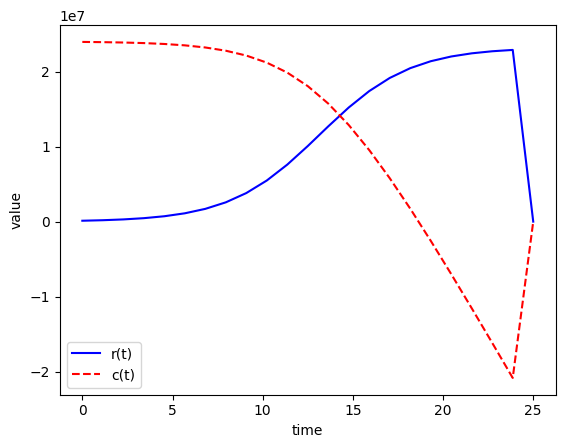
\includegraphics[width = 0.8\textwidth]{images/ode_problem2.png}
		\caption{Kết quả của mô hình}
	\end{figure}
\end{flushleft}
% section đề_xuất_phương_án (end)

% chapter bài_toán_2 (end)

\newpage

\chapter{Bài toán 3} % (fold)
\label{cha:bài_toán_3}

\section{Tiếp cận và giải quyết bài toán} % (fold)
\label{sec:tiếp_cận_bài_toán}
\begin{flushleft}
	Với bài toán này, nhóm chúng tôi quyết định sử dụng một mô hình khác với \textcolor{blue}{\hyperlink{chapter.2}{Bài toán 2}} để giải quyết vấn đề này. Có thể xem \textcolor{blue}{\underline{\href{https://github.com/XuananLe/MathModelingContest/blob/main/APM_TMH_V2/Problem3.ipynb}{Problem3.ipynb}}} của bài toán trên github của nhóm.
	\\[\baselineskip]

	Giới thiệu sơ qua về tập dữ liệu thì chúng ta chỉ có 21 điểm dữ liệu trải dài từ năm 2001 đến năm 2022. Nếu như chúng ta chỉ sử dựng 2 feature là lượng khí Co2 phát thải từng năm và diện tích rừng bị phá hủy từng năm thì chúng ta có thể thấy được rằng 2 feature này có mối quan hệ đơn giản nhưng không đủ phức tạp để đưa vào dự đoán. Vì vậy đội chúng tôi quyết định đề xuất thêm 2 feature nữa vào đó chính là GDP và mật độ dân số.
	\begin{itemize}
		\item GDP là thước đo tổng sản phẩm quốc nội của một quốc gia. GDP cao hơn thường đi kèm với tiêu dùng năng lượng cao hơn, dẫn đến phát thải CO2 cao hơn. Điều này là do GDP cao hơn thường đi kèm với tăng trưởng kinh tế, dẫn đến nhu cầu sử dụng năng lượng cao hơn cho các mục đích như sản xuất, vận tải và tiêu dùng.

		\item Mật độ dân số là số lượng người sinh sống trên một đơn vị diện tích nhất định. Mật độ dân số cao hơn thường đi kèm với nhu cầu sử dụng năng lượng cao hơn, dẫn đến phát thải CO2 cao hơn. Điều này là do mật độ dân số cao hơn thường đi kèm với đô thị hóa, dẫn đến nhu cầu sử dụng năng lượng cao hơn cho các mục đích như giao thông, sưởi ấm và làm mát.
	\end{itemize}

	Chúng ta hãy xem tập dữ liệu:
	\begin{figure}[H]
		\centering
		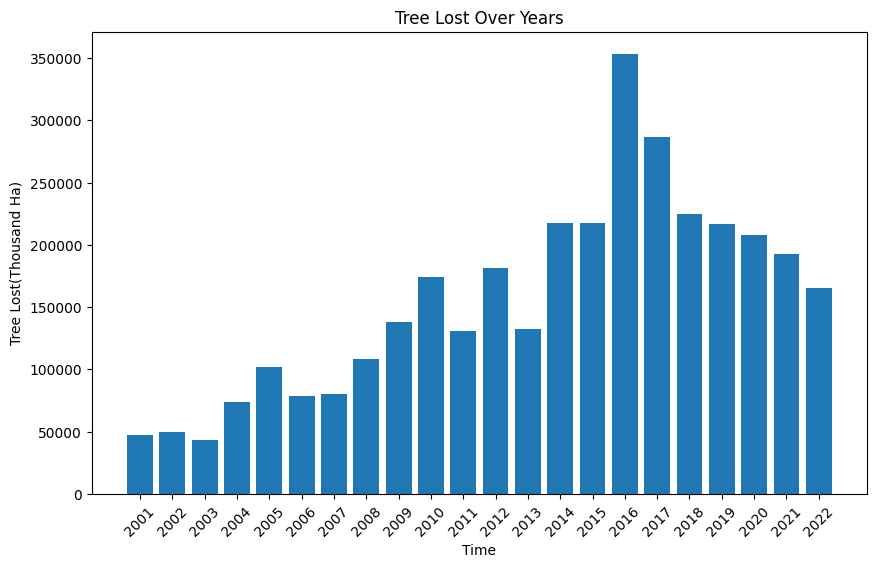
\includegraphics[width = 0.8\textwidth]{images/tree_loss_problem3.png}
		\caption{Diện tích rừng bị mất qua các năm}
	\end{figure}

	\begin{figure}[H]
		\centering
		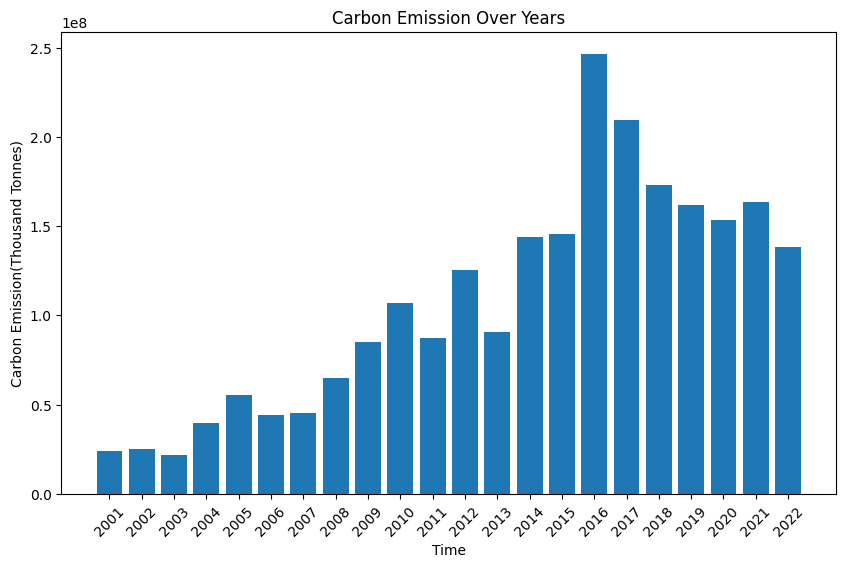
\includegraphics[width = 0.8\textwidth]{images/carbon_emission_problem3.png}
		\caption{Mức thải $CO_{2}$ qua các năm}
	\end{figure}

	\begin{figure}[H]
		\centering
		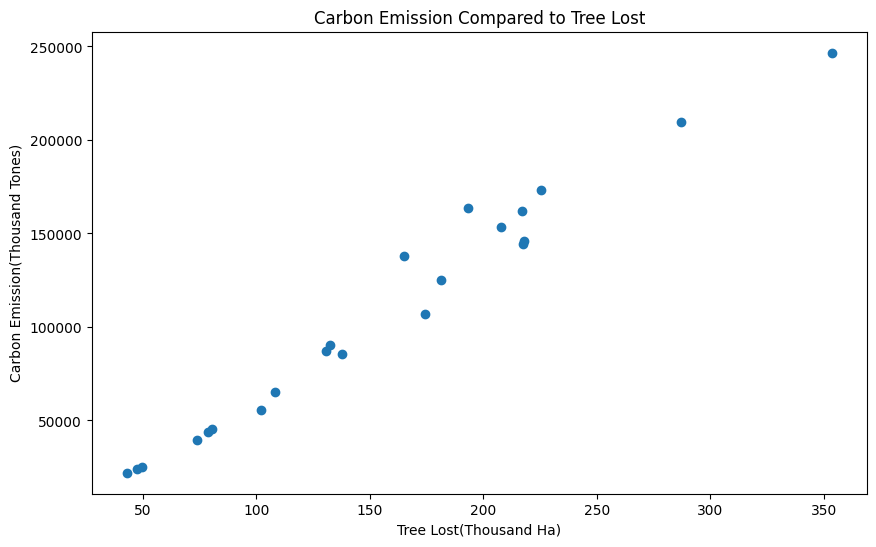
\includegraphics[width = 0.8\textwidth]{images/carbon_emission_v_tree_loss_problem3.png}
		\caption{Tương quan giữa lượng rừng bị mất và $CO_{2}$}
	\end{figure}

	Như chúng ta có thể thấy các cột dữ liệu có đơn vị khác nhau và độ lệch cũng rất lớn (Ví dụ như Co2Emission lại quá to hơn so với GDP của Việt Nam), điều này sẽ ảnh hưởng đến mô hình của chúng ta. Vì vậy chúng ta sẽ sử dụng Standard Scaler để chuẩn hóa dữ liệu. Standard Scaler là một kỹ thuật chuẩn hóa dữ liệu phổ biến nhất cho các thuật toán học máy. Nó có thể được sử dụng để chuẩn hóa dữ liệu đầu vào và cũng có thể được sử dụng trong việc chuẩn hóa dữ liệu đầu ra. Kỹ thuật này loại bỏ trung bình và chia tỷ lệ biến độc lập với độ lệch chuẩn của chúng.
	\\[\baselineskip]

	Standard Scaler chia tỉ lệ tất cả các giá trị của tập dữ liệu sao cho chúng có trung bình là 0 và độ lệch chuẩn là 1. Điều này giúp cho các tính toán của mô hình VAR trở nên ổn định hơn.
	\\[\baselineskip]

	Trong bài toán dự đoán lượng khí CO2 phát thải, việc sử dụng Standard Scaler có thể giúp cho mô hình VAR dự đoán chính xác hơn. Bởi vì các biến độc lập trong tập dữ liệu của bạn có thể có các đơn vị đo lường khác nhau và các phạm vi giá trị khác nhau. Việc sử dụng Standard Scaler sẽ giúp các biến độc lập có cùng một phạm vi giá trị, điều này sẽ giúp mô hình VAR học các mối quan hệ giữa các biến độc lập và biến phụ thuộc một cách chính xác hơn.
	\\[\baselineskip]

	Công thức chuẩn hóa dữ liệu của Standard Scaler như sau:
	$$
		x_{scaled} = \frac{(x - \gamma)}{\sigma}
	$$

	Trong đó:
	\begin{itemize}
		\item $x$: giá trị gốc.

		\item $x_{scaled}$: giá trị chuẩn hóa.

		\item $\gamma$: giá trị trung bình của tập dữ liệu.

		\item $\sigma$: độ lệch chuẩn của tập dữ liệu.
	\end{itemize}

	Đây là kết quả thu được:
	\begin{figure}[H]
		\centering
		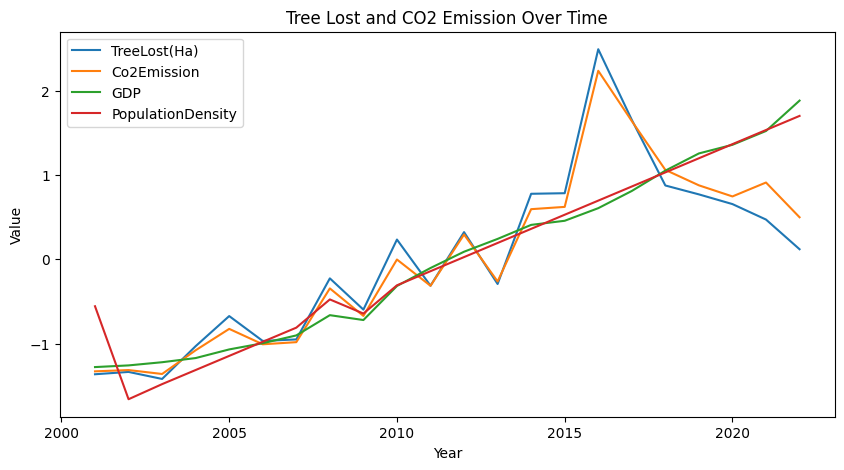
\includegraphics[width = 0.8\textwidth]{images/standard_scaler.png}
		\caption{Tập dữ liệu sau khi được chuẩn hóa}
	\end{figure}

	Theo như đề bài, chúng tôi sẽ đi dự đoán về chạy mô phỏng các kịch bản khác nhau để có thể dự đoán được diện tích rừng trong vòng từ 10, 20, 30, 50 và 100 năm tiếp theo.  Đây là bài toán về chuỗi thời gian (time-series). Có 1 số các phương pháp để có thể dùng để áp dụng như sau:
	\begin{itemize}
		\item Mô hình dự báo chuỗi thời gian: Các mô hình ARIMA (AutoRegressive Integrated Moving Average) hoặc các biến thể của nó thường được sử dụng để mô hình hóa và dự đoán chuỗi thời gian. Chúng dựa vào các mẫu thay đổi trong dữ liệu để dự đoán các giá trị tương lai. Phương pháp chính của ARIMA là xác định các tham số  chính : p (phần tự hồi quy), d (cấp số học của việc chuyển đổi dữ liệu), và q (phần trung bình trượt). Các tham số này xác định qua việc sử dụng các kỹ thuật như kiểm tra ACF (hàm tự tương quan) và PACF (hàm tự tương quan riêng). Chúng tôi đã thử phương pháp này và đường dự đoán quá lệch chuẩn so với đường thực tế như ảnh dưới đây.
		\begin{figure}[H]
			\centering
			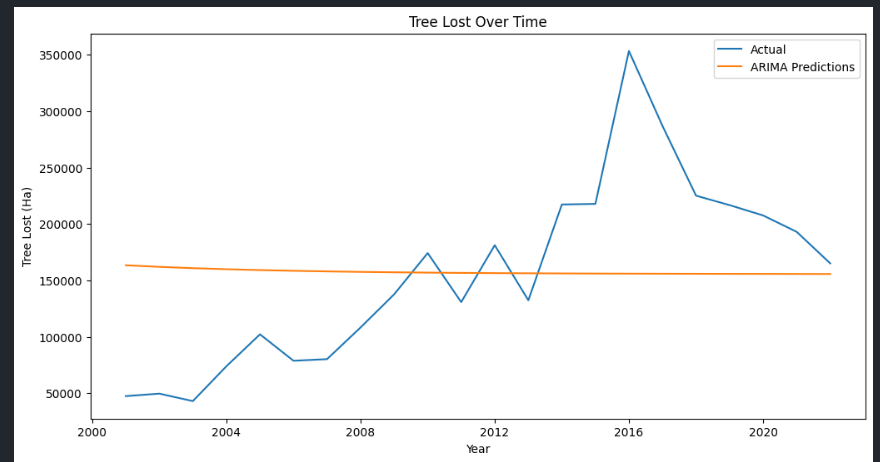
\includegraphics[width = 0.8\textwidth]{images/ARIMA.png}
			\caption{Kết quả thuật toán ARIMA}
		\end{figure}

		\item Mạng nơ-ron hồi quy (RNN) và LSTM: Đối với các chuỗi thời gian có sự phụ thuộc dài hạn và mô hình học tập từ dữ liệu lịch sử, các mạng nơ-ron hồi quy (RNN) và mạng nơ-ron hồi quy dài hạn (LSTM) có thể mang lại hiệu suất tốt. Tuy nhiên, chỉ với 20 điểm dữ liệu thu thập được (Xét từ năm 2001 - 2022) trong bài toán này, chúng tôi nghĩ rằng các mô hình này sẽ không hoạt động tốt và có khả năng overfit nếu như chúng ta cố gắng cho số epochs hoặc độ phức tạp của mạng neural network tăng lên.
	\end{itemize}

	Tại đây, chúng tôi quyết định sử dụng thuật toán Vector Auto Regression (VAR). VAR là một mô hình hồi quy tự hồi quy tích lũy. Nó dựa trên giả định rằng dữ liệu chuỗi thời gian có thể được mô hình hóa bằng một quá trình MA hoặc AR, hoặc cả hai. VAR có thể xử lý tốt các biến độc lập tuyến tính, nhưng nó có thể gặp khó khăn với các biến độc lập phi tuyến tính. Mục đích của chúng ta là để tối ưu hàm mất mát.
	$$
		J(p, q, \theta) = \sum\limits_{t = 1}^{T} \left(y_{t} - \sum\limits_{i = 1}^{p} \alpha_{i}y_{t - i} - \sum\limits_{j = 1}^{q} \beta_{j}x_{t - j} \right)
	$$

	Trong đó:
	\begin{itemize}
		\item $p$, $q$: số lượng tham số tự hồi quy trong mô hình VAR.

		\item $\alpha_{i}$ và $\beta_{j}$: các tham số tự hồi quy trong mô hình VAR.

		\item $x_{t}$: giá trị của biến độc lập tại thời điểm t.

		\item $y_{t}$: giá trị của biến phụ thuộc tại thời điểm t.
	\end{itemize}

	Đây là kết quả của mô hình sau khi thử với kịch bản 5 năm:
	\begin{figure}[H]
		\centering
		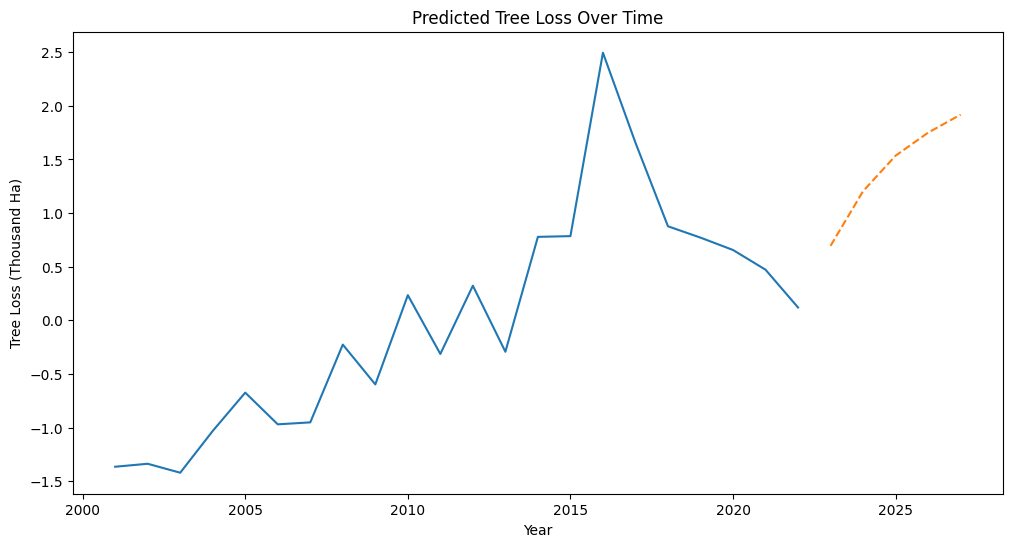
\includegraphics[width = 0.8\textwidth]{images/VAR_5.png}
		\caption{Thuật toán VAR sau 5 năm}
	\end{figure}

	Đây là kết quả của mô hình sau khi thử với kịch bản 20 năm:
	\begin{figure}[H]
		\centering
		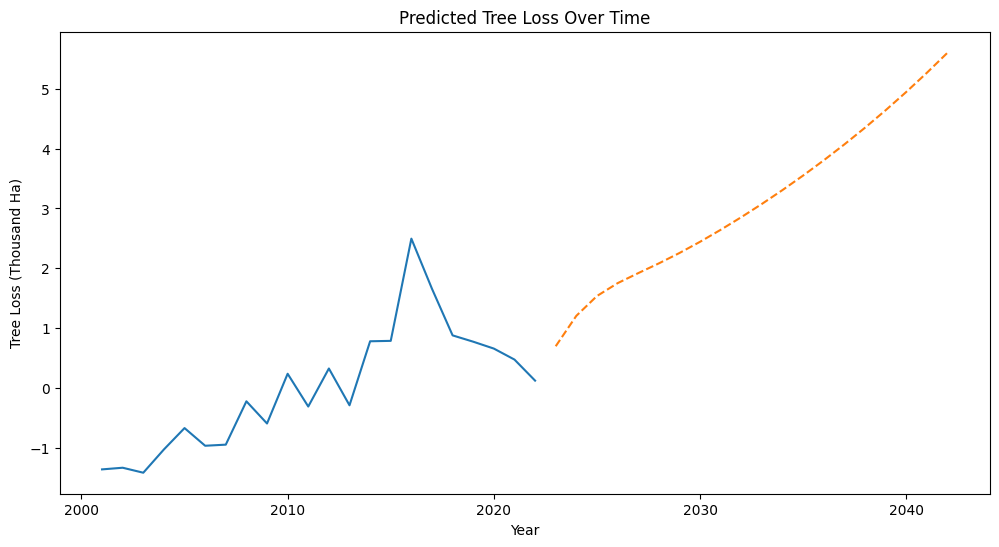
\includegraphics[width = 0.8\textwidth]{images/VAR_20.png}
		\caption{Thuật toán VAR sau 20 năm}
	\end{figure}
\end{flushleft}
% section tiếp_cận_bài_toán (end)

\section{Đánh giá mô hình} % (fold)
\label{sec:đánh_giá_mô_hình}
\begin{flushleft}
	Giá trị của "ADF Statistic" (Augmented Dickey-Fuller Statistic) là -6.138, và giá trị "p-value" là 8.08e-08, hay nói cách khác, rất gần bằng 0. Điều này có thể được hiểu như sau:
	\begin{itemize}
		\item \textbf{ADF Statistic}: Giá trị âm lớn cho thấy mạnh mẽ về việc bác bỏ giả thuyết null, tức là chuỗi có tính đơn vị gốc (unit root). Trong trường hợp này, chúng ta có thể kết luận rằng chuỗi số dư (residuals) có tính ổn định (stationary).

		\item \textbf{p-value}: Giá trị này rất nhỏ, ít hơn mức ngưỡng thông thường như 0.05 hoặc 0.01. Điều này cũng chỉ ra rằng chúng ta có đủ bằng chứng để bác bỏ giả thuyết null.
	\end{itemize}

	\textbf{Kết luận}: Với một giá trị ADF như vậy và một p-value rất nhỏ, chúng ta có thể tin tưởng rằng chuỗi số dư (residuals) của mô hình là ổn định, hay nói cách khác, đã đạt được tính chất không dừng (stationarity). Điều này là một dấu hiệu tích cực cho thấy mô hình của chúng ta đã khá tốt trong việc nắm bắt các mẫu dữ liệu trong tập dữ liệu huấn luyện. Tuy nhiên, điều này không đảm bảo mô hình sẽ hoạt động tốt trên dữ liệu mới hoặc tương lai.

\end{flushleft}
% section đánh_giá_mô_hình (end)

% chapter bài_toán_3 (end)


\chapter*{Các đường dẫn tham khảo} % (fold)
\addcontentsline{toc}{chapter}{Các đường dẫn tham khảo}
\begin{flushleft}
	\begin{enumerate}
		\item Repository của nhóm. \url{https://github.com/XuananLe/MathModelingContest}

		\item Các nguồn dữ liệu sử dụng trong báo cáo này:
		\begin{itemize}
			\item \url{https://rainforests.mongabay.com/deforestation/archive/Vietnam.htm}

			\item \url{https://data.worldbank.org/}
		\end{itemize}
	\end{enumerate}
\end{flushleft}
% chapter các_đường_dẫn_tham_khảo (end)

\end{document}